\documentclass[draft]{book}
\usepackage{amsmath}
\usepackage[acronym]{glossaries}
\usepackage[backend=biber, natbib=true]{biblatex}
\usepackage{tikz}
\usetikzlibrary{arrows,positioning,shapes.geometric, calc}
\usepackage{amsthm}
\usepackage{graphicx}
\usepackage{caption}
\usepackage{subcaption}
\newtheorem{mydef}{Definition}
\usetikzlibrary{positioning}
\usepackage{setspace}
\linespread{1.5}

\bibliography{/home/robert/Documents/library.bib}
\title{The Genetics of Aggressive Behavior}
\author{Robert Milan Porsch}
\date{\today}
% Evo history
\newacronym{rhp}{RHP}{Resource Holding Power}
\newacronym{rv}{RV}{Resource Value}
\newacronym{adhd}{ADHD}{Attention Deficit Hyperactivity Disorder}
\newacronym{sst}{SST}{Sexual Selection Theory}
\newacronym{vntr}{VNTR}{Variable Number Tandem Repeat}


% Methods twins
\newacronym{sem}{SEM}{Structural Equation Model}
\newacronym{mz}{MZ}{monozygotic}
\newacronym{dz}{DZ}{dizygotic}

% Methods gwas
\newacronym{gwas}{GWAS}{Genome Wide Association Study}
\newacronym{snp}{SNP}{Single Nucleotide Polymorphism}
\newacronym{ld}{LD}{Linkage Disequilirium}
\newacronym{pca}{PCA}{Principle Component Analysis}
\newacronym{pc}{PC}{Principal Component}
\newacronym{fdr}{FDR}{False Discovery Rate}
\newacronym{gcta}{GCTA}{Genome-wide Complex Trait Analysis}
\newacronym{maf}{MAF}{Minor Allele Frequency}
\newacronym{skat}{SKAT}{sequence kernel association test}


%\tikzexternalize % for faster compilation

\begin{document}
\maketitle
\chapter{Introduction}
\label{cha:introduction}

% dramatic entry
Aggressive behavior has potential beneficial and harmful consequences for the aggressor.
While aggression caries a serious risk of bodily harm for the aggressor, it also has the potential to increase access to resources and higher social status.
The nature and cause of such behavior has always been of interest to social and biological focused researchers and much scientific effort has been spent to investigate the various different facets of this complex behavior.
While previous research has been focused on environmental as well as biological causes of aggressive behavior, here I will solely focus on potential biological mechanisms of human aggression.
Specifically I will investigate potential genetic causes of human aggressive behavior via a variety of different statistical methods.

The first chapter of this thesis will review the existing literature in regards to the definition and forms of aggression, as well as evolutionary theories and known genetic risk factors associated with this complex behavior.
Subsequently, I will give an overview of the statistical methods used within this thesis.
Chapter 3 describes my investigation of over 28,000 twin pairs to examine the longitudinal heritability of childhood aggression.
The next chapter describes the exploration of specific molecular genetic markers associated with risk taking and aggression in over 150,000 unrelated individuals.
Afterwards, in chapter 5, I will examine the genetic overlap of various traits with aggressive behavior.
Chapter 6 will outline a newly-developed method to test for distributional differences of rare mutations between aggressive and non-aggressive subjects.
Finally, I will discuss my findings in detail and outline future research directions.

\section{Definition of Aggression}
\label{sec:overview_of_reseach_in_aggression}

One can define human aggression as a behavior intended to cause physical or emotional harm to others~\cite{Anderson2002}.
However, this definition is rather incomplete.
It is also important to consider the unwilling participation of the victim as well.
Hence behaviors in which the target does not intend to avoid the aggressive behavior, such as in sexual masochism~\cite{Berkowitz1993,Baumeister1989,Baron2007,Geen2001}, should not be considered  aggressive acts.
Thus the motivation of the victim to avoid such harm plays an important role in the definition of aggression.  
Therefore I will use the following working definition:
\begin{mydef}[Aggression]\label{def:aggression}
	`Aggression is the delivery of an aversive stimulus from one person to another, with intent to harm and with an expectation of causing such harm, when the other person is motivated to escape or avoid the stimulus'~\cite{Geen2001}
\end{mydef}

While aggression is most commonly associated with physical harm, Definition~\ref{def:aggression} also includes a broader spectrum.
Nonviolent behavior, like spreading gossip, damaging a victim's property either due to emotional anger or as a planned action to gain an advantage to a higher goal.
This large spectrum of aggression makes it necessary to specify the broader dimension of this behavior.

\subsection{Forms of aggression}
\label{sub:forms_of_aggression}

One can separate aggressive behavior into \textit{affective aggression} and \textit{instrumental aggression}.
While \textit{affective aggression} is characterised as emotional, impulsive, thoughtless, and unplanned behavior, \textit{instrumental aggression} is defined as a planned and proactive behavior to obtain a certain higher goal~\cite{Berkowitz1993,Geen2001}.
This distinction has been extended by a number of similar concepts, such as \textit{reactive/proactive} and \textit{offensive/defensive} aggression.
While these terms have slightly different meaning, depending on situation and field of research, the general concept remains similar~\cite{Geen2001, Blanchard2005b}.
In psychology, for example, the terms \textit{affective aggression} and \textit{instrumental aggression} have been established, but more recently authors have used the terms \textit{reactive} and \textit{proactive} aggression~\cite{Geen2001}.
Thus aggressive action in response to a provocation, such as in self-defence and in anger, is \textit{reactive aggression} while planned, unprovoked aggression is called \textit{proactive}.

However, despite the differences in terminology, it is important to emphasise the strong negative emotional state of \textit{affective/reactive} aggression.
This state, often described as \textit{anger}, launches and guides affective aggression  and is often caused by some form of provocation~\cite{Geen2001}.
Nevertheless, \citet{Frijda1994} suggested that \textit{affective/reactive aggression} is not necessarilly impulsive.
In some situations, a delay between provocation and aggressive response is observed. 
In particular, long term grudges, or \textit{hatreds}, are preoccupations which go beyond the initial provocation but remain deeply emotional.
Thus I will use the term \textit{impulsive aggression} to refer to impulsive, emotionally-guided, aggressive behavior.

In contrast, \textit{instrumental/proactive aggression} is characterized by the absence of an emotionally strong goal to cause harm.
For example, the use of gossip and bad-mouthing of a colleague in order to obtain higher chances of receiving a promotion is done in a planned manner with the aim of a higher goal.
However, it is often difficult to distinguish actions into affective and instrumental aggression since both forms are not mutually exclusive.
\citet{Geen2001} gave the example of a mother who uses corporal punishment to modify her child's behavior, while still reacting in anger when observing the undesired child's behavior,
hence mixing a planned aggressive act towards a higher goal with an emotional, angry state.

Both forms of aggression, affective and instrumental, can be either physical or verbal.
While physical aggression in humans is homologous to other animals, verbal aggression, a form of \textit{indirect}, \textit{relational}, and \textit{social}, aggression, is relatively distinct to humans~\cite{Archer2005}.
These verbal behaviors cause harm to others by gossiping, spreading rumors, or excluding other from social groups.
While the terms \textit{indirect}, \textit{relational}, and \textit{social} aggression have been differently conceptualized in the past~\cite{Archer2001}, they are expressed in common behaviors and can be contrasted to physical, \textit{direct}, aggression.
Hence the terms are more similar than distinct and I will therefore proceed to call all them \textit{indirect} aggression in order to distinguish it more from the physical, more direct aggressive behavior~\cite{Archer2005}.

Research in animals has often used a slightly different terminology.
Investigations often have distinguished between \textit{offensive} and \textit{defensive} aggression~\cite{Blanchard2005b}.
Similar to \textit{affective} aggression, \textit{offensive} attacks arise from a response to a threat to the animal's resources, thus are the response to a certain provocation.
These resources could be sexual partners, food, social status, or, in the case of humans, money.
On the other hand, \textit{defensive} aggression is a response to a direct threat to the subject's life, a concept closely related to \textit{instrumental} aggression.
While this distinction might hold in mice and rats, the separation between \textit{offensive} and \textit{defensive} aggression is more blurred in primates, including humans.
For example, humans are known to hunt lions and other predators.
In contrast to non-predators, these animals are, for the most part, not eaten which would suggest a form of defensive aggressive behavior.
However, within most human cultures killing a large predator is seen to enlarge one's social status by showing strength and courage towards the others,
a behavior which is an \textit{offensive} action.

However,~\citet{Blanchard2005b} suggest, while the separation between \textit{offensive/affective}  and \textit{defensive/instrumental} might be blurred in humans, the distinction holds in general.
Indeed, the authors suggest that rather insufficient analysis and not a disconnection between animal and human behavior are responsible for the blurred distinction.
However, \citet{Blanchard2005b} provide little evidence for their claims and one can argue that the complexity of human society makes a comparison between subcategories of aggressive behavior across species especially difficult. 
Nevertheless, animal studies have provided valuable insight into aggressive behavior and I will outline a number of experimental findings in animal studies in later sections.

To conclude, one can distinguish between \textit{affective} and \textit{instrumental} forms of human aggression which can be  either \textit{direct} or \textit{indirect}.
Research in non-humans has often distinguished between \textit{offensive} and \textit{defensive} forms of aggression.
I will next consider evolutionary theories in regards to aggression in humans and animals alike.
I will show that aggressive behavior has a strong evolutionary background and that genes which regulate such behavior are under stabilizing selection.

\section{Evolutionary Theories}
\label{sec:evolutionary_theories}

Historically, research on aggression has been divided into nurture versus nature~\cite{Archer2009}. 
Proponents of the nurture side have argued that aggressive behavior is caused by environmental influences, while supports of the nature side of the discussion supported the idea that differences in the genetic architecture are able to explain considerable individual differences in aggressive behavior.
Today's view is less polarized and acknowledges that both nature and nurture play a crucial part in aggression.
While not disregarding the environmental aspect of aggression I will mostly focus on the genetic and biological mechanisms of aggressive behavior.
In the following section I will outline evolutionary concepts helpful in explaining and understanding individual differences in aggression. 

Evidence for a long history of human aggression can be found in  paleontological findings of broken bones, rips and smashed skulls, unexplainable without the consideration of weaponry force.
Occasional findings of weapon fragments in skeletal rib cages suggest that violence and aggression has been part of the human evolutionary history. 
\citet{Buss1997}, one of the founders of evolutionary psychology, suggested that all psychological mechanisms and behavior, including aggression, can ben explained by the evolutionary principle of selection.  
These mechanisms are aimed to solve specific adaptive problems.
Hence some variants of those behaviors and psychological mechanisms might solve certain problems better than others, thus improving overall fitness.
This results in the preservation, replication, and spreading of theses variants through a population~\cite{Buss1997}.

\citet{Buss1997} suggested \textit{seven} adaptive problems to which aggressive behavior might be an evolutionary solution.
For example, \textit{co-opt the resources of others}, which can be defined as the use of physical or psychological force to obtain resources held by another individual or group, can give the aggressors significant advantages in terms of survival and reproduction.
These resources could mean food, water, land, or sexual partners.
An example of this can be seen in aggressive behavior of children.
\citet{Campbell1995} noted that aggression among toddlers is often about resources, such as toys, suggesting that this behavioral adaptation is a deeply rooted evolutionary strategy.

Aggression can also be useful in \textit{defending against an attack}.
Since attacking aggressors are a serious threat to valuable resources,
aggression can be an effective strategy in defending against individuals or groups.
Furthermore, it can be also an adaptive strategy to foster a reputation that would deter potential aggressors~\cite{Buss1997},
thus avoiding the potential cost of a physical conflict while defending one's resources.

Another evolutionary benefit of aggression can be found in the social hierarchies in groups.
For example, men who win fights and defeat opponents gain power and status in many societies~\cite{Hill1996}.
The gain in social status can be beneficial in accessing resources and mates~\cite{Archer2009}.
Indeed, hierarchical order in social groups is often established by means of aggressive behavior which enables high-ranked individuals priority access to food and patterns~\cite{Lindenfors2011}. 
However, aggression can also result in a decline in status.
\citet{Buss1997} suggested for example that a physical conflict between two professors in a faculty meeting would result in a decline in reputation.
Thus displays of aggression are not acceptable in all social situations or always helpful in achieving a goal.

In the context of reproduction one should consider aggression towards the same-sex separate of male-female aggression.
Aggression towards same-sex individuals is sometimes aimed to reduce their social status and therefore make them less attractive to the other sex~\cite{Buss1990}.
Hence inflicting damage on a rival directly translates to an increased benefit to the aggressor.
In addition to aggression towards same-sex individuals, aggression is also prevalent towards the opposite sex.
For example, aggression can be used to deter a long-term mate from infidelity~\cite{Daly1982}.
However, also here aggression can have negative consequences in the form of retaliation.
A husband might be reluctant to use aggression towards his wife when she is living close to a number of brothers and a powerful father.
Indeed, a study in Madrid, Spain, found that women who had a higher density of genetic kin in and around Madrid were less likely to be victim of domestic violence~\cite{Figueredo1995}.
Furthermore, expressing aggression towards another individual sheers energy away from other actives, such as hunting and foraging, and also carries a high risk of injury and death~\cite{Packer1995}.  
This increased cost is also reflected in the conflict resolving methods applied across many animals and humans.
For example, two competing male red deer may begin their confrontation by roaring repeatedly.
If this does not resolve the conflict both will walk side-by-side while attempting to make themselves look as large as possible.
Only the last stage involves a physical confrontation, potentially causing severe injuries~\cite{Clutton-Brock1979}.
These behaviors, aimed to resolve conflicts without the use of raw force, demonstrates the large costs of physical aggression.
However, it  also shows that animals and humans alike are able to avoid those costs by threatening the use of physical force.
\citet{Maxson2005} suggested that if the resource holding potential (\acrshort{rhp}), which is defined as the ability to win a physical fight over resources,  as well the resource value (\acrshort{rv}) itself, are the same for both contestants, conflicts will usually escalate.

Negative consequences might also be present when aggression is used to gain a higher social status.
In a study~\cite{Packer1995} on 138 female baboons in the Gombe National Park in Tanzania high-ranking females showed shorter inter-birth intervals as well as higher offspring survival rates.
Thus one would expect higher life-time reproductive success in baboons with overall higher social rank across their lifetime.
However, the authors were not able to associate reproductive success with mean lifetime rank.
\citet{Packer1995} suggested that this inconsistency can be explained by considering that higher ranked females are also more likely to suffer  miscarriages.
These stress-related failures in reproduction can be seen as a counter-force to a potential arms race among female baboons.
Hence the induced aggression by competing for higher social status carries the cost of significant risk of miscarriages.

Therefore, the increase in fitness due to aggressive behavior, either as a direct gain in resources or higher social status, is balanced by large risks, such as injuries, death, and reduced reproduction.
This would indicate that aggression is under stabilizing selection (see figure~\ref{fig:stab}).

\begin{figure}[hp]
	\centering
	\scalebox{0.6}{\tikzstyle{box} = [rectangle, rounded corners, minimum width=3.5cm, minimum height=1cm,text centered, draw=black]
\begin{tikzpicture}
	\draw[line width=6, gray] (-7,0)-- (0,0) --(7,0);
	\draw[gray, fill=gray] (-1,-2)-- (0,0) --(1,-2) --(-1,-2);

	%Cost
	\node (injury) [box, fill=red!80] at (-5,0.6)  {Reproductive Cost};
	\node (grooming) [box, fill=red!70, above of=injury] {Foraging};
	\node (repo) [box, fill=red!60, above of=grooming] {Parental care};
	\node (foraging) [box, fill=red!50, above of=repo] {Grooming};
	\node (parCare) [box, fill=red!40, above of=foraging] {Injury risk};

	%Benefit
	\node (mat) [box, fill=green!80] at (5,0.6)  {Mating priority};
	\node (res) [box, fill=green!70, above of=mat] {Resource access};
	\node (def) [box, fill=green!60, above of=res] {Predator defense};
	\node (surv) [box, fill=green!50, above of=def] {Survival};
	\node (dom) [box, fill=green!40, above of=surv] {Social Dominance};

\end{tikzpicture}
}
  \caption[Stabilizing selection of aggressive behavior]{Stabilizing selection of aggressive behavior (as in~\citet{Anholt2012}).
  The benefit of aggressive behavior is countered by its cost, thus maintaining a stable level of aggressive behavior within the population}\label{fig:stab}
\end{figure}

Furthermore, same-sex and male-female aggression is not equally balanced among the two sexes and nearly all mammals display sex differences in the expression of aggression, both
qualitative, the type of aggression, as well as quantitative, the amount of aggression.
In general males are more likely to exhibit physical aggression than female.
These sex differences have been discussed in the context of \acrfull{sst}~\cite{Archer2004,Anderson2002,Archer2009}. 
Sexual selection is concerned with how a member of one sex chooses another individual from the other sex, as well as the competition between members of the sex over access to the other~\cite{Darwin1859}.
In most mammals the more competitive sex is the male~\cite{Archer2009}. 
\citet{Trivers1972} suggested that these sex differences can be explained by the limited parental investment by males in many species.
Parental investment is the amount of resources a parent invests into his or her offspring to increase its survival and reproduction~\cite{Archer2009}.
The theory was first suggested by~\citet{0198504403} and proposes that a male can minimize his parental investment in favor in producing a greater number of offspring.
In contrast, many female mammals have a large obligatory parental investment, such as gestation and delivery.
This greater parental investment makes it more important to remain alive in order to raise the offspring,
\citet{Campbell1999} suggested that this discrepancy resulted in more risk-averse behaviors in female.
This would further predict that while direct aggression is quantitatively imbalanced between the sexes, indirect aggression is expressed in both males and females to an equal level due to its lower cost.
Indeed, multiple studies have found no sex differences in indirect aggressive behavior~\cite{NoelCard2008}.
Hence sexual selection can be used to explain sex differences in humans and animals alike.

The above outlined cross-species and evolutionary history of aggressive behavior suggests that inherited biological factors play a key role.
I have shown that aggression, while having large benefits for the aggressor, also caries significant drawbacks.
In the following section I will outline specific genetic aspects associated with aggression.


\section{Biological Mechanisms}
\label{sec:biological_mechanisms}

As outlined in Section~\ref{sec:evolutionary_theories}, aggressive behavior is present in a number of species which indicates that this particular behavior is, from an evolutionary view, relatively old.
However, most findings in regards to the genetics of aggressive behavior comes from animal studies due to the ethical considerations of experimental studies in humans.
Hence previous research has made use of comparative genetics to gain insight into the genetic mechanisms of human aggression.
Comparative genetics is the use and analysis of genomic information across species to identify and relate genes with phenotypes~\cite{Maxson2003}.
A cross species perspective enables one to examine overlapping genes which might affect a particular behavior.
This not only allows one to identify genes involved in aggression across species but also enables consideration of gene-environment interactions.

\subsection{Investigative approaches}
\label{sub:investigation_approaches}

\citet{Maxson2005} further proposed three general approaches to investigate the genetic architecture of aggressive behavior.
(1) One can identify genes by mapping their sequence to different forms of aggression (see my own study in Chapter~\ref{ha:assocation_study_in_agggressive_behavior_and_risk_taking}).
(2) Another approach is to alter the genetic code of experimental organisms, such as rats and mice, to test for the effects of different genes on aggression.
(3) Last, one can measure the rate of gene expression within the brain in association with an aggressive phenotype.
Only in recent years options (1) and (3) have been made possible due to progress in the sequencing of human and animal genomes.
Option (2) has the highest scientific validity due to the use of randomized control trials, a method only available in nonhuman animals.
However, one can also add a fourth and fifth category.
Indeed, investigation of DNA methylation in order to uncover the epigenetic mechanisms of aggressive behavior is gaining more traction.
DNA methylation is a biological control mechanism by cells to control gene expression.
While studies on DNA methylation in human aggression have been only recently  conducted~\cite{VanDongen2015a}, this new field of study is potentially promising in investigating the genetic mechanisms of aggression.
Further, while~\citet{Maxson2005} only described molecular methods, one can also make use of twin pairs.
Twin studies make use of the genetic similarity (or dissimilarity) of dizygotic and monozygotic twins, since dizygotic twins, and siblings for that matter, share 50\% of their genetic makeup with their brother or sister, while monozygotic twins share 100\%.
This enables one to estimate the genetic contribution of aggressive behavior in humans.
These studies have been a popular method to investigate the genetic contribution of a variety of different phenotypes and I will outline a detailed description of this particular method in Section~\ref{sec:twin_based_studies}. 
Most twin studies have estimated the genetic contribution to aggressive behavior between 50\% and 80\%~\cite{Porsch2016}.
While these estimates give a broad understanding about the importance of genetic factors  to aggression, twin studies are unable to inform about specific genes or genetic markers.

\subsection{Identification of \textit{MAOA}}
\label{sub:identification_of_MAOA}

One well known genetic characteristic of aggressive behavior was discovered when analysing a rather large Dutch family~\cite{Brunner1993}.
In particular, male members of this family were known for their aggressive behavior, including arson, attempted rape, and other forms of aggression.
Genomic analysis revealed that individuals had a deficient monoamine oxidase due to a point mutation in the \textit{MAOA} gene, suggesting a causal link between \textit{MAOA} and aggressive behavior.
Interestingly, this causal link has been replicated multiple times in humans~\cite{Huang2004,Manuck2000} as well in mice~\cite{Cases1995} and monkeys~\cite{Newman2005}.

Within the following section I will outline previously uncovered specific genetic associations in human and nonhuman animals alike.
Further I will discuss previous findings in regards to gene-gene and gene-environment interactions. 

\subsection{Genetic Associations in nonhuman animals}
\label{sub:genetic_associations_in_animals}

Genetic analysis in animals has a number of advantages.
First, one is able to make direct manipulation of the genome in question, and second, one is able to quantify aggressive behavior more easily.
For example, aggression in mice can be measured by counting the number of attacks the animal performs when placed in a situation which involves social confrontation with another mouse.

A number of studies have investigated the effect of different neurotransmitters on aggressive behavior, mostly using mice~\cite{Anholt2012}.
For example, studies which focused on serotonin demonstrated differences on the type of receptors activated.
Mice whose \textit{5-HT1B} receptor was knocked out demonstrated hyper-aggressive symptoms while those mice which were treated with \textit{5-HT1A} receptor antagonist displayed reduced aggression~\cite{Saudou1994,Bell1994}.

Furthermore, the knock-out of the non-functional nuclear receptor \textit{NR2E1} has been shown to result in a hyper aggressive state in mice~\cite{Young2002}.
Also a knockout of \textit{NOS1} in mice showed an increased level of aggressive behavior.
Interestingly, this particular knockout not only resulted in a hyper-aggressive state but also in a behavior which can be described as a relentless attack on opponents who had surrendered or showed no interest in a confrontation.
Hence these mice demonstrated a qualitatively different aggressive behavior compared to other mouse knock-outs.
Further, within these animals one could observe clear sex differences.
While male mice showed the above-described hyper aggressive state, female mice showed a reduced aggressive behavior against male invaders~\cite{Gammie1999,Nelson1995}, demonstrating a sex-specific genetic regulator of aggression.

\subsubsection{Gene-Gene interaction in nonhuman animals}
\label{ssub:Gene-Gene_Interaction_in_nonhuman_animals}

In their review,~\citet{Anholt2012} pointed to a number of gene-gene interactions which seem to regulate these single gene effects.
For example, the knockout of \textit{NR2E1} had different effects depending on the genetic background~\cite{Young2002}.
While the mouse models C57BL/6J-frc and B6129F1-frc both displayed increased levels of aggression, C57BL/6J-frc demonstrated significantly more aggressive behavior,
 suggesting that the knock-out resulted in a different effect depending on the genetic background.
Identification of further gene-gene interactions in humans, however, remains difficult due to the lack of sufficient sample size in many genome-wide association studies.

\subsection{Genetic Associations in Humans}
\label{sub:genetic_associations_in_humans}

Genetic association studies in humans commonly face difficulties in obtaining large enough sample sizes and therefore lack statistical power.
Thus previous studies have focused on only a handful of selected genes to investigate the genetic architecture of human aggression.
For example, Alzheimer patients who are homozygous for the \textit{apolipoprotein E $\epsilon 4$} allele have been reported to express more aggressive behavior~\cite{Craig2004,VanDerFlier2006}.
However, these findings could not be replicated in a study with larger sample size~\cite{Hollingworth2006}.
Similarly, studies on the catechol-O-methyl transferase gene (COMT) in schizophrenia have associated a single polymorphism with aggression~\cite{Hirata2013,Calati2011}, but the sample sizes of these studies were small.


%TODO there is more!!!!!!

\subsubsection{Gene-Gene interactions in humans}
\label{ssub:Gene-Gene_interactions_in_humans}

Similar to the findings in mice, a single-gene association study of $1,308$ patients with attention deficit/hyperactivity disorder (ADHD) and a criminal history demonstrated that a single polymorphism in the \textit{NOS-I} gene was associated with impulsivityy, hyperactivity, and aggression.
While this study was able to confirm smaller studies analysing the same gene, the combined sample size was rather small,
thus one should be caution in respect to \textit{NOS-I} since genome-wide analysis are preferred.

The discovery of the importance of \textit{MAOA} put other neurotransmitters into focus, including serotonin~\cite{Murphy2008}, dopamine, norepinephrine, and GABA~\cite{Marino2005,Miczek2002}.
For example,~\citet{Hohmann2009} identified an association between a \acrfull{vntr} and externalizing behavior in the dopamine D4 receptor (\textit{DRD4}) gene.
Interestingly, subjects who also had a mutation in the serotonin transporter \textit{SLC6A4}, specifically in the serotonin-transporter-linked polymorphic region (\textit{5-HTTLPR}), showed high levels of aggressive behavior.
This behavior was not present if only one of the two mutations were present.
Hence this is a rare display of a gene-by-gene interaction, also called epistasis~\cite{Anholt2012}, in a behavioral phenotype.

To conclude, genetic analysis in humans has shown multiple different potential genes implicated in human aggression.
Most prominently \textit{MAOA} as well as \textit{DRD4} in combination with \textit{SLC6A4}.
However, studies in humans have so far only focused on a few sets of candidate genes due to the high costs associated with an analysis of the whole genome.

\section{Genes and the Environment}
\label{sec:gene_environment_interactions}

Many behavioral phenotypes depend on the surrounding environmental conditions (see Figure~\ref{fig:plasticity}).
For example, in threatening situations, one might be prone to exhibit more aggression compared to non-threatening circumstances. 
On the other hand, gene-environment interactions is when the phenotypical expression of one genotype depends on environmental stimuli (see Figure~\ref{fig:gene_env_interaction}).
Interestingly, aggressive behavior is one of the few behavioral phenotypes were previous research has shown gene-environment interactions.

\begin{figure}[!htp]
  \centering
  \begin{subfigure}[t]{0.4\textwidth}
    \centering
    \resizebox{\linewidth}{!}{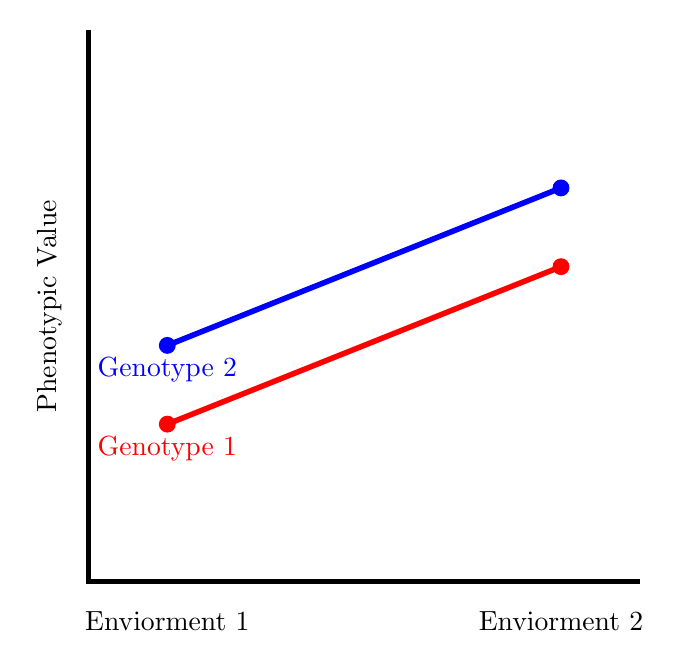
\begin{tikzpicture}
	% axes
	\draw[line width=2, black] (7,0)  -- (0,0) --(0,7);

	% interaction
	\draw[line width=2, red] (1,2) node[below] {Genotype 1}-- (6,4);
	\draw[red, fill=red] (1,2) circle (0.1cm);
	\draw[red, fill=red] (6,4) circle (0.1cm);

	\draw[line width=2, blue] (1,3) node[below] {Genotype 2}-- (6,5);
	\draw[blue, fill=blue] (1,3) circle (0.1cm);
	\draw[blue, fill=blue] (6,5) circle (0.1cm);

	% text
	\node at (1,-0.5) {Enviorment 1};
	\node at (6,-0.5) {Enviorment 2};
	\node[rotate=90] at (-0.5,3.5) {Phenotypic Value};
\end{tikzpicture}
}
    \caption{Phenotypic plasticity}\label{fig:plasticity}
  \end{subfigure}
  \begin{subfigure}[t]{0.4\textwidth}
    \centering
    \resizebox{\linewidth}{!}{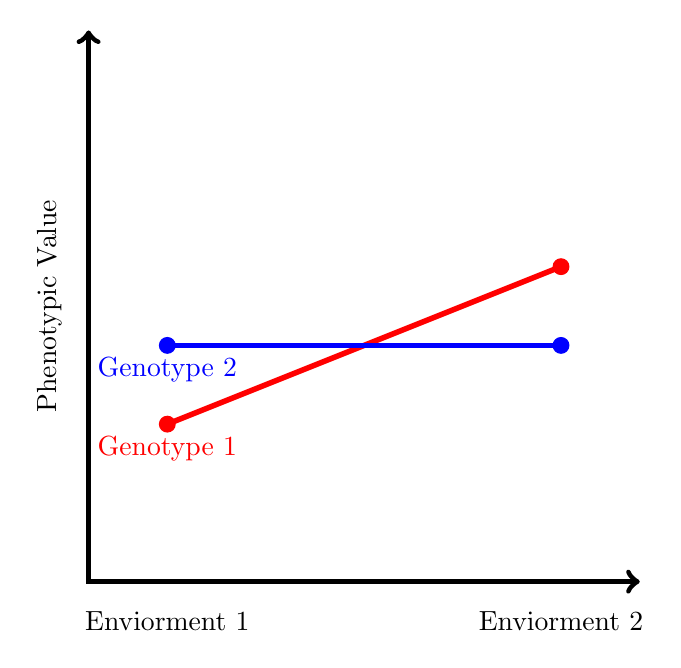
\begin{tikzpicture}
	% axes
	\draw[line width=2, black, <->] (7,0)  -- (0,0) --(0,7);

	% interaction
	\draw[line width=2, red] (1,2) node[below] {Genotype 1}-- (6,4);
	\draw[red, fill=red] (1,2) circle (0.1cm);
	\draw[red, fill=red] (6,4) circle (0.1cm);

	\draw[line width=2, blue] (1,3) node[below] {Genotype 2}-- (6,3);
	\draw[blue, fill=blue] (1,3) circle (0.1cm);
	\draw[blue, fill=blue] (6,3) circle (0.1cm);

	% text
	\node at (1,-0.5) {Enviorment 1};
	\node at (6,-0.5) {Enviorment 2};
	\node[rotate=90] at (-0.5,3.5) {Phenotypic Value};
\end{tikzpicture}
}
    \caption{Gene-by-enviornment interaction}\label{fig:gene_env_interaction}
  \end{subfigure}
  \caption[Gene-Environment Interactions]{Different interactions between genes and the environment. 
    The colors represent different genotypes. 
    (a) Different environments result in the same effect independent of genotype.
    (b) The effect of the environment is genotype-specific}\label{fig:env_interactions}
\end{figure}

\subsection{\textit{MAOA} interactions}
\label{sub:maoa_interactions}

The effects of \textit{MAOA} and serotonin transporters have been shown to be dependent on the individual's previous experiences.
\citet{Caspi2002} showed in a sample of $499$ male children that some children who were maltreated developed anti-social behavior.
This effect seemed to be moderated by a mutation in \textit{MAOA}.
Children with higher expression of \textit{MAOA} were less likely to suffer from anti-social behavior following maltreatment.
These results were later replicated by a number of similar studies~\cite{KimCohen2006}.
However, not all studies were able to replicate these findings.
\citet{Anholt2012} suggested that the failure to replicate can be explained by the low statistical power of some of the studies as well as diversity of the used samples, including sex, age, and ethnicity.
Indeed, other studies have found a more complex picture of \textit{MAOA}-environment interactions.
\citet{Huang2004} for example showed that this gene-environment interaction is male-specific, and \citet{Weder2009} demonstrated that extreme cases of maltreatment did not result in varying effects of later anti-social behaviors.
Nevertheless, it is still unclear how maltreatment in childhood results in anti-social behavior later in life and how \textit{MAOA} is moderating this effect.
Furthermore, most studies had little statistical power,
thus large scale population data is necessary to confirm this gene-by-environment interaction.

\subsection{\textit{5-HTTLPR} interactions}
\label{sub:httlpr_interactions}
Interestingly, also the serotonin transporter has been subject to investigations regarding gene-environment interactions.
However, the results are less conclusive.
A polymorphism in \textit{5-HTTLPR} has been found to result in higher levels of aggressive behavior in  people with depression~\cite{Gonda2011} and intellectual disabilities~\cite{May2010}, while not demonstrating associations in non-affected subjects.
In the review by~\citet{Anholt2012}, the authors suggested these associations as a further indicator of gene-environment interactions.
However, given the small sample size of the studies, other possibilities might explain these findings.
For example shared genetic mechanism between depression, intellectual disabilities and aggression, could also explain the increased effect of polymorphism in \textit{5-HTTLPR} on aggressive behavior. 
Nevertheless, the identification of gene-environment interaction within aggressive behavior suggest a complicated genetic architecture underlying aggressive behavior.
\bigskip

In conclusion, I have outlined definitions of aggressive behavior and evolutionary theories and concepts surrounding it.
Further, I have reviewed and described previous research into specific genetic aspects of aggression in human and nonhuman animals alike.
In addition I have shown that previous research has also demonstrated considerable gene-environment interaction within aggression.
In the following chapter I will describe methods used to investigate the genetic architecture of human aggression.

\documentclass[../header.tex]{subfiles}
% Evo history
\newacronym{rhp}{RHP}{Resource Holding Power}
\newacronym{rv}{RV}{Resource Value}
\newacronym{adhd}{ADHD}{Attention Deficit Hyperactivity Disorder}
\newacronym{sst}{SST}{Sexual Selection Theory}
\newacronym{vntr}{VNTR}{Variable Number Tandem Repeat}


% Methods twins
\newacronym{sem}{SEM}{Structural Equation Model}
\newacronym{mz}{MZ}{monozygotic}
\newacronym{dz}{DZ}{dizygotic}

% Methods gwas
\newacronym{gwas}{GWAS}{Genome Wide Association Study}
\newacronym{snp}{SNP}{Single Nucleotide Polymorphism}
\newacronym{ld}{LD}{Linkage Disequilirium}
\newacronym{pca}{PCA}{Principle Component Analysis}
\newacronym{pc}{PC}{Principal Component}
\newacronym{fdr}{FDR}{False Discovery Rate}
\newacronym{gcta}{GCTA}{Genome-wide Complex Trait Analysis}
\newacronym{maf}{MAF}{Minor Allele Frequency}
\newacronym{skat}{SKAT}{sequence kernel association test}

\begin{document}
\chapter{General Methodology}
\label{cha:methods_applied_in_genetic_studies_on_humans}

The investigation of underlying genetic architectures of human traits is limited to non-experimental studies and one can broadly distinguish between two types.
Twin studies and association studies.

Twin studies make use of monozygotic and dizygotic twin pairs to estimate the contribution of genetic and environmental components of a trait.
In contrast, association studies make use of recently developed molecular methods to identify specific genetic variations within the human genome associated with a specific trait.

Within this section I will describe commonly used methods in both twin and molecular based association studies.
I will further describe methods used to estimate heritability and genetic correlations.

\section{Twin based studies}
\label{sec:twin_based_studies}

Twins have always been of special interest to scholars.
Indeed already Hippocrates has been reported to be interested in twins at around 5th century BCE\@.
While his original accounts is lost the Roman politician and author Cicero described Hippocrates's observations of two ill brothers, suspected to be twins, with similar identical disease progression~\cite{Cicero44BC}.
Thus providing the first writen account of a twin study.

Much later Francis Galton was one of the first persons to use twins in order to investigate the effect of genes and the environment on human behavior~\cite{Rende1990}.
However, only when~\citet{Simens1924} discovered the two distinct types of twins, namely \acrfull{mz} and \acrfull{dz} twins, twin studies became an established instrument in the investigation of genetic factors in humans.

MZ twins develop from a single fertilized egg and therefore share all of their genetic variations.
On the other hand, \acrfull{dz} twins develop from two fertilized eggs and share only 50\% of their genetic variations.
This distinction forms the basis of all twin studies and allows to state structural equations relating observed trait and theorized underlying genetic and environmental effects.

In addition, Genetic effects can be further distinguished between additive genetic effects (A) which represents the accumulated effect of all genetic variations and dominant (D) effects which represents interaction on the same genetic locus.
Environmental components are differentiated into shared environment (C) and unique environment (E).
Therefore the total variance of a any particular trait is $P = A+D+C+E$.

Since one can assume different correlations between MZ and DZ twin pairs one can estimate components of $P$.
While the correlations between twins within C and E are the same in both MZ and DZ twins, namely $1$ and $0$ respectively.
In contrast, MZ twins have a correlation of $1$ for both A and D, while DZ pairs have a correlation of $\frac{1}{2}$ and $\frac{1}{4}$ respectively.
Therefore differences within MZ twins can be attributed to E alone.
Further, when we assume that DZ and MZ twins are exposed to the same degree of similarity within their environment, the differences in similarity between MZ and DZ twins is an estimate of $A+D$.
This is also called Falconer's formula (see Formula~\ref{eq:falcon}) and can be used to estimate heritability, or the relative importance of genetic effects.

\begin{align}
  h^2 &= 2(r_{MZ}-r_{DZ})\label{eq:falcon} \\ 
  C &= r_{MZ} - h^2  \\
  E &= 1 - h^2 + c^2  
\end{align}

However, while the above is attractive it its simplicity, today's twin studies use \acrfull{sem} to model genetic and environment effects.
SEMs are more flexible in modeling specific hypothesis, are able to test for sex differences as well are able to handle multivariate data~\cite{Rijsdijk2002}.

Figure~\ref{fig:ace} displays such a classical path based model.
Variables within an SEM can be separated into latent and observed variables.
Additive genetic (A), common environment (C) and unique environment (E) are so called latent variables.
These variables are not directly observed but are inferred from actual measured variables.
Observed variables are commonly displayed in cornered boxes.
The double headed arrows represents the correlations among A and C.
The causal paths $a$, $c$, and $e$ represents the to estimate effect of the components on the trait $T$.
The square of these estimates are the variance components of A, C and E respectively.
However, effects of $D$ cannot be simultaneously estimated with $A$, and two separate models need to be constructed.

\begin{figure}[htpb]
  \centering
  \scalebox{0.6}{%\usetikzlibrary{external}
%\tikzset{external/system call={latex \tikzexternalcheckshellescape -halt-on-error
%		-interaction=batchmode -jobname "\image" "\texsource";
%		dvips -o "\image".ps "\image".dvi ;
%		ps2eps "\image.ps" "\image".eps}}
%\tikzexternalize
%\newcommand{\at}{\makeatletter @\makeatother}
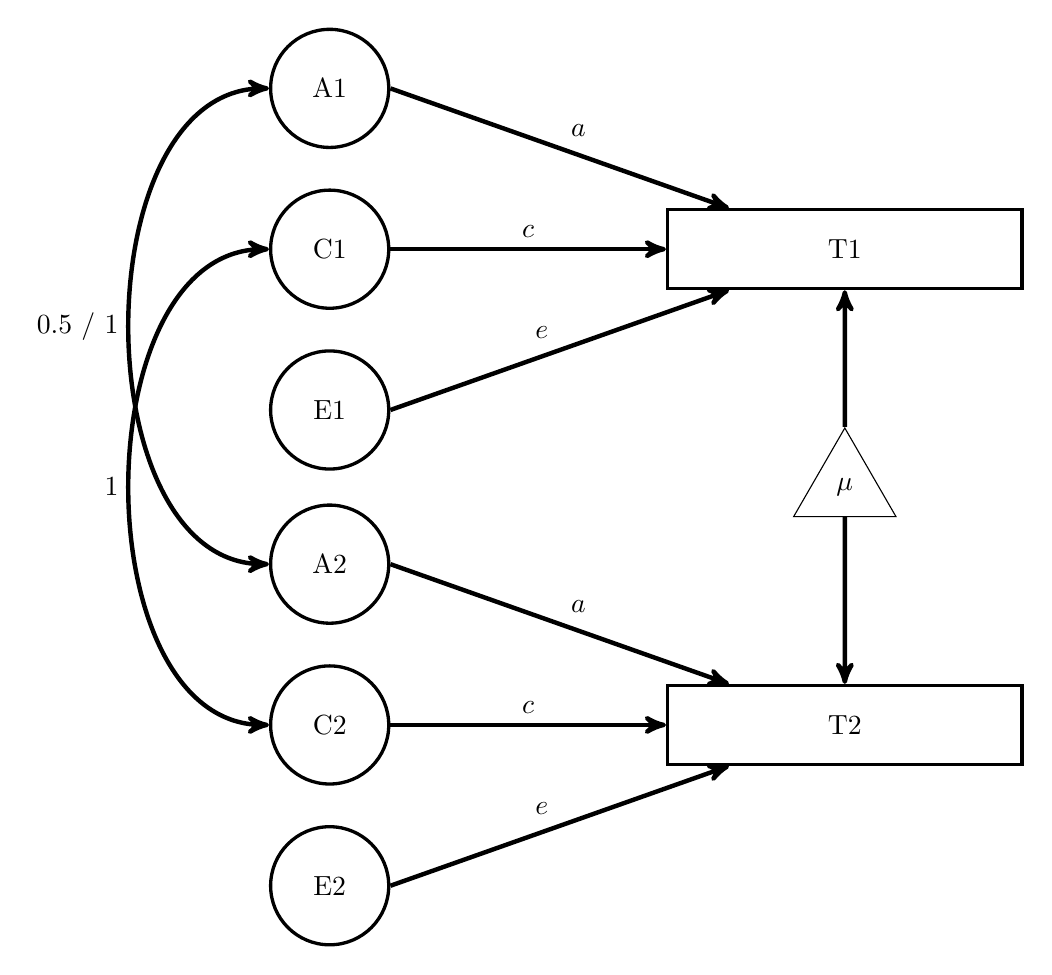
\begin{tikzpicture}[auto,node distance=.5cm,
    latent/.style={circle,draw,very thick,inner sep=0pt,minimum size=15mm,align=center},
    manifest/.style={rectangle,draw,very thick,inner sep=0pt,minimum width=45mm,minimum height=10mm},
    paths/.style={->, ultra thick, >=stealth'},
    twopaths2/.style={<->, ultra thick,bend left=90, >=stealth'},
    twopaths1/.style={<->, ultra thick,bend right=90, >=stealth'},
    mean/.style={draw, regular polygon, regular polygon sides=3, node distance=1cm, minimum height=15mm}
]

% Define observed variables
\node [manifest] (T1) at (0,0) {T1};
\node [manifest] (T2) [below=of T1, below=5cm of T1]  {T2};


% Define latent variables
\node [latent] (C1) [left=3.5cm of T1] {C1};
\node [latent] (C2) [left=3.5cm of T2] {C2};
\node [latent] (A1) [above=of C1] {A1};
\node [latent] (A2) [above=of C2] {A2};
\node [latent] (E1) [below=of C1] {E1};
\node [latent] (E2) [below=of C2] {E2};

\node [mean] (mu) at($(T1)!0.5!(T2)$)  {$\mu$};

% paths to T1/T2
\draw [paths] (A1.east) to node {$a$} (T1);
\draw [paths] (A2.east) to node {$a$} (T2);
\draw [paths] (C1.east) to node {$c$} (T1);
\draw [paths] (C2.east) to node {$c$} (T2);
\draw [paths] (E1.east) to node {$e$} (T1);
\draw [paths] (E2.east) to node {$e$} (T2);

% path from mean
\draw [paths] (mu.south) to node [right] {} (T2);
\draw [paths] (mu.north) to node [right] {} (T1);

% variance
\draw [twopaths1] (A1.west) to node  [bend left=90, left]{0.5 / 1} (A2.west);
\draw [twopaths2] (C2.west) to node  [bend right=90, left]{1} (C1.west);

\end{tikzpicture}
}
  \caption{
    Basic ACE model.
    This basic model contains the latent variables A, C and E for twin 1 and 2, as well as the observed variable T with the mean $\mu$.
  }\label{fig:ace}
\end{figure}

The covariance matrix of the model in Figure~\ref{fig:ace} is therefore
\begin{equation}
  cov(MZ) = 
  \begin{pmatrix}
    a^2 + c^2 + e^2 & a^2 + c^2 \\
    a^2 + c^2 & a^2 + c^2 + e^2
  \end{pmatrix}
\end{equation}
and 
\begin{equation}
  cov(DZ) = 
  \begin{pmatrix}
    a^2 + c^2 + e^2 & \frac{1}{2}a^2 + c^2 \\
    \frac{1}{2}a^2 + c^2 & a^2 + c^2 + e^2
  \end{pmatrix}
\end{equation}

Modern SEM software is able to estimate parameters by minimising the goodness-of-fit statistic between the observed and predicted covariance matrices~\cite{Boker2011}.
Most commonly this is done via a maximum-likelihood function.
Further, the overall goodness-of-fit of the model relatively to a perfect fit, meaning that parameters are considered as `free' and their maximum-likelihood estimate will equal the sample covariance, are measured by a likelihood ratio square statistic ($\chi^2$).
Therefore, should we fail to reject the null hypothesis that our model in Figure~\ref{fig:ace} is different from a perfect fitted model we have reason to assume that our genetic model fits the data.

The use of SEM allows for great flexibility and a variety of models to be estimated.
In the past few decades numerous twin studies on a variety of traits have been performed.
It not only allowed to test for the differences in the genetic architecture between the sexes but also to look at how the influence of genetic factors change over age.
However, due to the new advancement in acquiring genetic information of individual more research has been shifted to \acrfull{gwas}.
Hence, in the next section I will outline the methods applied GWAS\@.

\section{Association studies of common variants}
\label{sec:association_studies_of_common_variants}

Large scale genomic association studies have enabled researchers to investigate specific genetic factors associated with a certain trait.
Hence, while twin studies were only able to give an estimate of the total contribution of genetic factors on a phenotype, association studies are able to elucidate the specific molecular basis of complex traits.
Specifically, these genome wide association studies utilize common \acrfull{snp} and other genetic variations, to identify specific genetic markers associated with a certain trait.
Common variants are usually genetic variations with a frequency $\ge 1\%$, also called \acrfull{maf}.

\paragraph{What is an \acrfull{snp}}
\label{par:what_are_snp}
SNPs are variations within the genome at a specific position and underly differences in traits and disease susceptibility. 
For example, the replacement of the nucleotide cytosine (C) with tymine at a certain position within a stretch of DNA is considered a \acrfull{snp}.
Most SNPs have no or little effect on specific traits.

Association analysis of common genetic variants are usually only applied to investigate potential genetic markers of common traits and disorders.
This is due to the hypothesised differences in the genetic architecture influencing common and rare disorders.

This hypothesised difference between common and rare diseases originates from one of the early successes in human genetics.
Specially the identification of multiple genetic markers in \textit{CFTR} which are responsible for cystic fibrosis.
This was made possible by a technique called \textit{linkage analysis}, which made use of the segregation of genetic markers across multiple families affected by the disorder~\cite{Kerem1989}.
However, while this method was initially successful with a number of other rare disorders, such as Huntington, common disorder, such as heart diseases, psychiatric disorders as well as other, fared not that well.  
Implying that common and rare disorders have a different genetic architecture~\cite{Hirschhorn2005a}.
Therefore leading to the development of the common disease common variant hypothesis.

\subsection{Common disease common variant hypothesis}
\label{sub:common_versus_rare_genetic_variants}

The common disease common variant hypothesis suggests that common disorders are affected by genetic variations which are also common in the population.
This hypothesis, while simplistic, has some profound implications.

First, it is unlikely that common variants will have a high penetrance and are the lone disease causing mutations.
For example, a common variants with a frequency of 45\% that directly cause a disorder would mean that also 45\% of the population would be affected by the disease.
This is unlikely to be the case and it is more likely that a given SNP only has a small effect of the disease.
For example, an SNP might only slightly alter the gene expression of a particular gene and increase the overall risk for a disease.
Implying that the correlation between the allele frequency and disease prevalence will be low.
Thus, suggesting that common variants are unlikely to have a high penetrance.

This in turn also implies that multiple common variants affect a common disorder.
For example, twin studies have estimated the heritability of aggressive behavior at 50\%.
If a single SNP has only a small effect on the phenotype, then the total genetic risk must be distributed across multiple common genetic variants.
Figure~\ref{fig:rare_comon} displays the spectrum of genetic affects and allele frequency.

\begin{figure}[htpb]
  \centering
  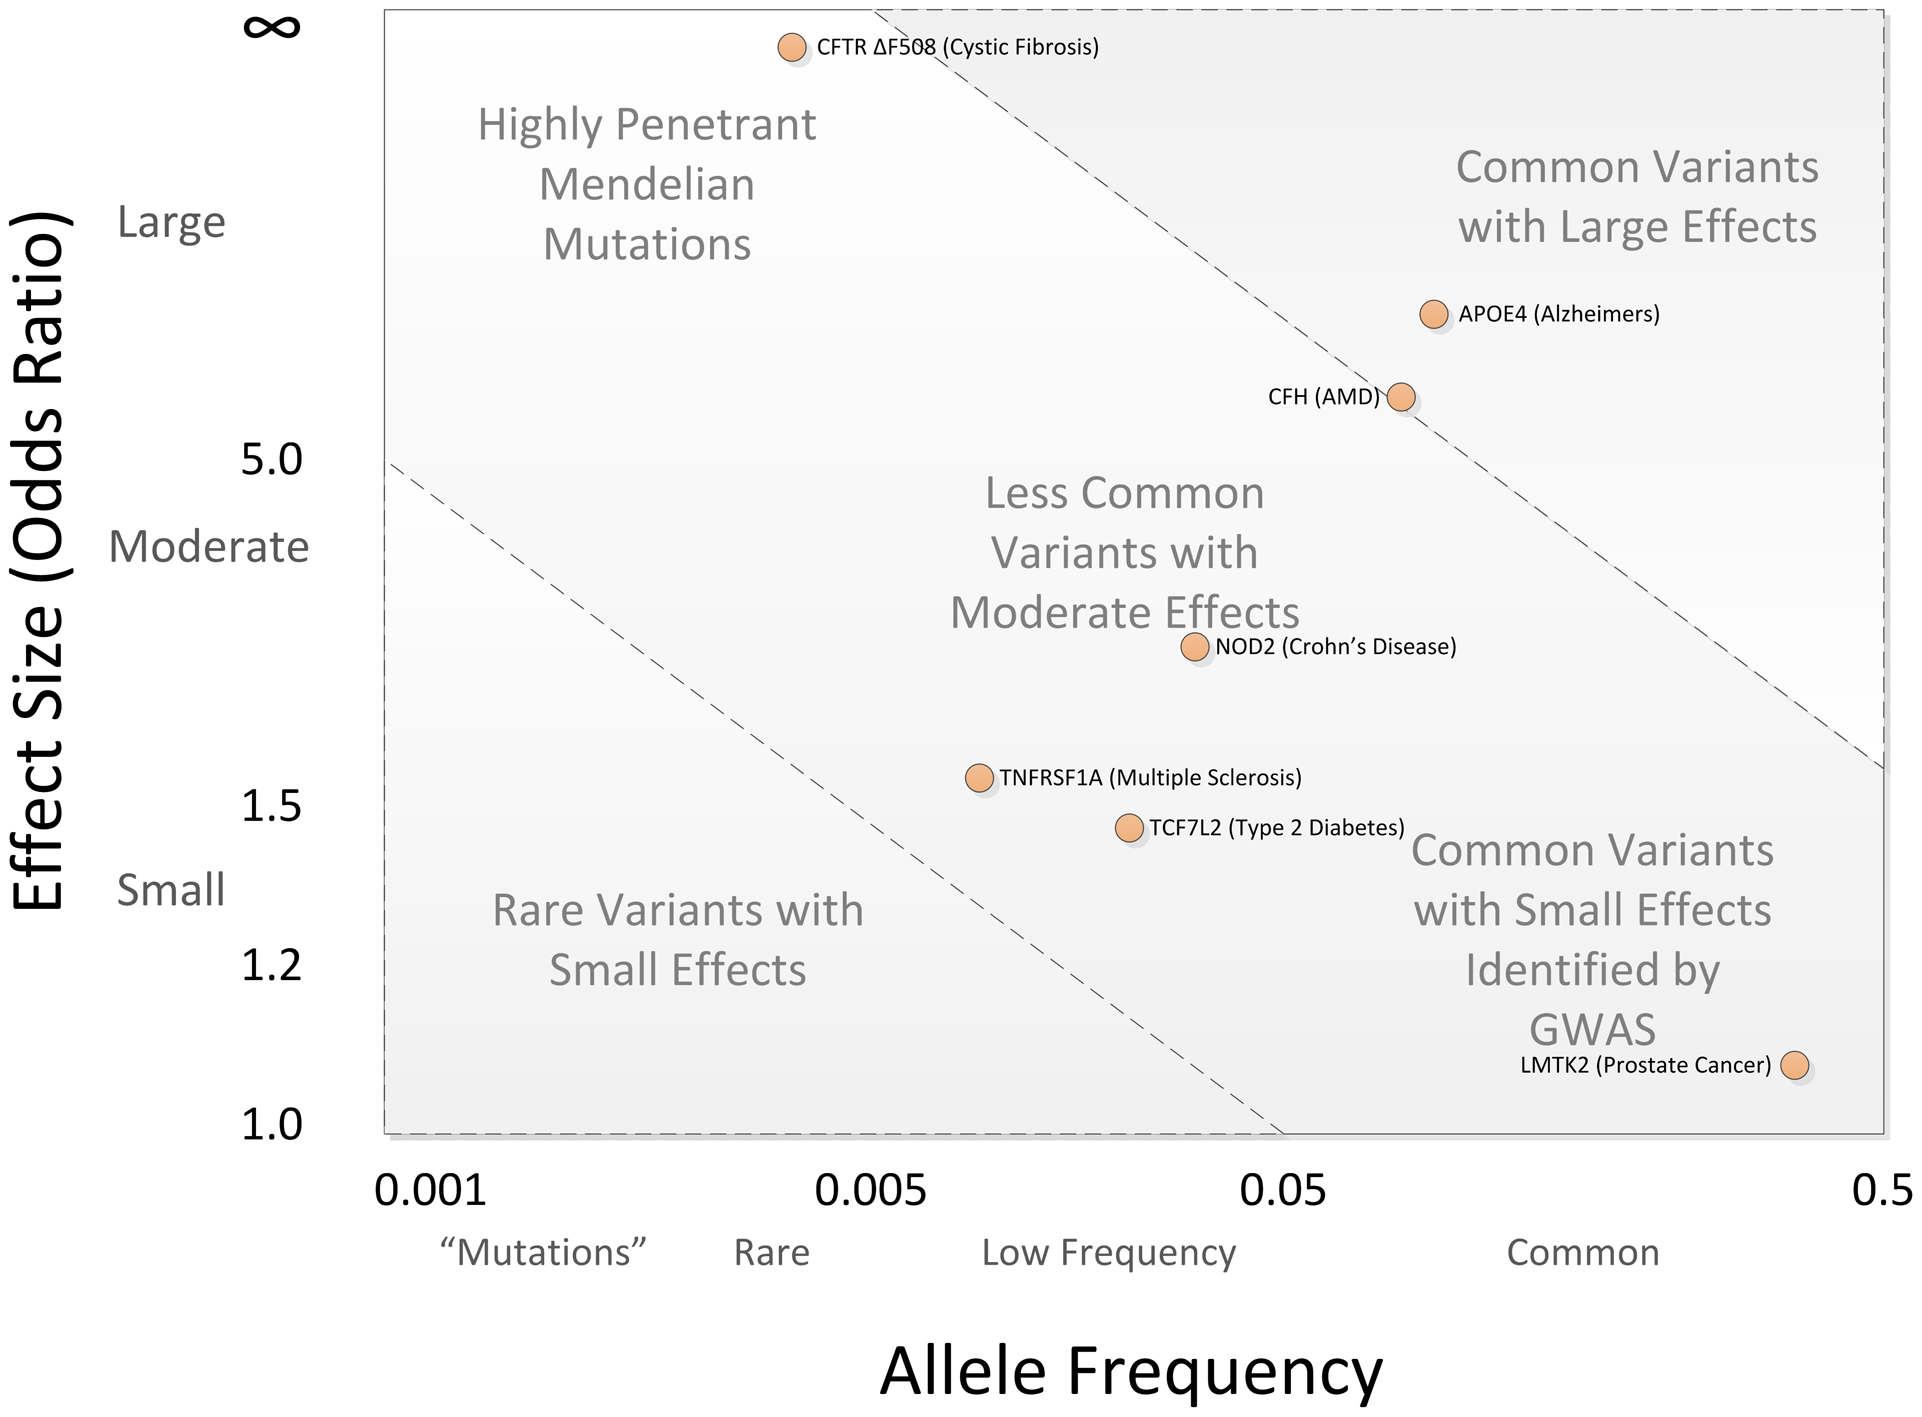
\includegraphics[width=0.8\linewidth]{{figure/journal.pcbi.1002822.g001}.png}
  \caption{Spectrum of Disease Allele Effects~\cite{Bush2012}.}\label{fig:rare_comon}
\end{figure}

Overall the common disease common variant hypothesis has been tested numerous times~\cite{Bush2012}.
Most common SNPs identified in the last 10 years are of low effect and most common disorders have multiple risk alleles~\cite{Welter2014}.
Therefore suggesting that the hypothesis holds true. 
However this does suggest that all genetic contributions to a common disorder are due to common variants alone.

\subsection{Linkage Disequilibrium}
\label{sub:linkage_disequilibrium}

Before explaining the concept of association studies in more detail it is important to mention \acrfull{ld}.
LD is `the nonrandom association of alleles at different loci'~\cite{Slatkin2008} and forms a marker of the population genetic mechanism that is at play within our genome.
For example, two loci are said to be in high LD when allele $A$ at one loci co-occurs with allele $B$ at a different loci at a higher frequency then one would expect if the two loci were independent.
Hence the level of LD can be quantified as $D_{AB}=p_{AB} - p_{A}p_{B}$ in which in which $p_{AB}$ is the frequency that $A$ and $B$ occurs together wile $p_A$ and $p_B$ is the frequency of $A$ and $B$ respectively.
If $D_{AB} \neq 0$ A and B are said to be in linkage disequilibrium, otherwise the two alleles are in linkage equilibrium ($D_{AB}=0$).
Nevertheless, $D_{AB}$ depends on the frequencies of the alleles in questions and are therefore not always convenient.
Therefore, LD between two loci is commonly measured in two different ways. 
That is $D'$ and $r^2$.
\citet{Lewontin1964} suggested to use
\begin{equation}\label{eq:dprime}
  D' = D/D_{\min}
\end{equation}
where 
\begin{equation*}
  D_{\min}= \begin{cases}
    \max\{-p_A p_B,\,-(1-p_A)(1-p_B)\} & \text{when } D < 0\\
    \min\{p_A (1-p_B),\,(1-p_A) p_B\} & \text{when } D > 0
  \end{cases} 
\end{equation*}
Alternatively, one can also use the correlation coefficient $r$ between the two loci 
\begin{equation}\label{eq:r2}
  r=\frac{D}{\sqrt{p_A(1-p_A)p_B (1-p_B)}}
\end{equation}
An important consequence for association studies is that an association between a trait and an allele is unlikely to be the actual causal SNP\@.
An association between an SNP and a trait can arise out of multiple reasons.
First, the association could represent the true effect and the particular SNP has a causal relationship on the trait in question.
Second, and more likely, the associated SNP is a proxy of the causal SNP since both are in high \acrshort{ld}.
Third, the association is a random fluctuation within the sample, and 
fourth the association is due to confounding errors such as population stratification or genotyping errors.

\subsection{Association test}
\label{sub:association_test}

The association between an SNP $g$ and a trait $y$, as well as additional covariates $\bm{U}$, of an individual $i$ can be expressed as a generalized linear regression model for a continuous and binary phenotype.
\begin{equation}
  g(E(y_i)) = \beta_0 + \beta_1g_i + \bm{\beta_u}\bm{U_i'} + \epsilon
\end{equation}
In which $\beta_0$ is the intercept (commonly ignored in GWAS settings) and $\beta_1$ the regression coefficient of a particular SNP\@.
The vector $\bm{\beta_u}$ of size $1\times p$ are the regression coefficients of $p$ covariates to adjust for potential confounding factors.
Possible confounding factors are population stratification, sex, genotyping chip and others.
The link function $g(.)$ is a logit function for binary traits, while for quantitative traits no transformation is used (identity link function). 

Genotypes of each SNP can be organized to represent dominant, recessive, multiplicative, as well as additive models.
For example, assuming at a given position the two genotypes are \textit{A} and \textit{a}.
In a dominant model having one or two copies of \textit{A} increases disease risk ($AA > Aa > aa$).
In contrast, a recessive model requires at least two copies of the risk allele ($AA > Aa = aa$).
The multiplicative model assumes a quadratic increase in risk.
If the risk of having the \textit{A} allele is $k$ than having two copies of the same allele is $k^2$.
An additive model assumes a linear increase in risk for each additional allele copy.
Thus if the risk of \textit{Aa} is $k$ then the risk doubles ($2k$) for \textit{AA}. 
Despite these different models GWAS commonly use an additive model only since it has appropriate statistical power to detect dominant effects as well.
Nevertheless, it is important to keep in mind that an additive model has  having reduced power for potential recessive effects~\cite{Bush2012}.

\subsection{Population Stratification}
\label{ssec:population_stratification}

Population stratification takes place when differences in the frequencies of alleles among cases and controls are not due to an causal relationship between the SNP and the trait.
Rather it is caused by ancestral differences across populations.
An association is affected by population stratification if the trait is more prevalent in one population while the allele frequencies vary across the populations.

Commonly one can adjust for population stratification by the usage of \acrfull{pca}.
PCA is a procedure which transforms a set of correlated variables into a set of linear uncorrelated once, called principle components (\acrshort{pc}).
The number of PC can be smaller or equal that of the number of initial variables and the first PC accounts for most of the variability in the set of correlated variables.
Each following PC explains the most variance constrained that it is orthogonal to the previous.
Using PCA on a matrix of genotypes results in a set of PCs which explain the genetic variation within the sample.
Given the sample is a mixture out of multiple populations with different ancestry the computed PCs will often have geographic interpretation.
Thus including PCs into the association model will adjust for population stratification arising due to differences in allele frequencies and disease prevalence.

\subsection{Multiple Testing}
\label{ssec:multiple_testing}

Testing a large amount of genetic variants without adjusting the significant threshold $\alpha$ results in a large number of falsely associated variants.
Therefore adjustments of the significant threshold is necessary.
For example, one could simply adjust $\alpha$ by the number of tests performed (Bonferroni threshold).
However, this would result in an overly conservative threshold and in a number of false negative associations~\cite{Benjamini1995} since computed test statistics are not independent due to LD\@.
Indeed,~\citet{Peer2008} estimated, based on data from the International Haplotype Map Consortium, the number of independent tests to be one million in Europeans and two million in African populations.
Therefore most GWASs have used a threshold of $5\times 10^{-8}$.
However, due to the introduction of larger sample sizes as well as better technology we are able to genotype variants with lower allele frequency.
This requires adjustment of the GWAS significant threshold since it also increases the number of independent tests.
Hence~\citet{Fadista2016} recently suggested to use $3\times10^{-8}$, $2\times10^{-8}$, $1\times10^{-8}$ for variants with $MAF\ge1\%$, $MAF\ge0.5\%$ and$ MAF\ge0.1\%$.

\acrshort{gwas} are useful in identifying molecular markers for traits and diseases.
While there are multiple possible confounding factors, such as population stratification, methods have been developed to approach these problems successfully.
However, usually GWAS do not deal with genetic variations with a frequencies below 1\%.

\section{Heritability and Genetic Correlation}
\label{sec:heritability_and_genetic_correlation}

As already described above, studies on twins were able to assess the heritability of traits by considering the inter-correlation among MZ and DZ twins.
Therefore, one would expect that the variance explained by all genetic variants combined would result in similar estimates.
Unfortunately, for many traits, this is not the case.
This is called the `Missing Heritability Problem'~\cite{Vineis2010} and a  number of reasons have been suggested for the discrepancy between estimates in twin studies and those in GWAS\@.

First, the assumptions in twin studies might be violated and estimates are too high.
In particular, studies on twins assume that the influences of shared environmental factors influences MZ and DZ twins to the same extend.
However, one can argue that MZ twins are treated by parents, teachers and peers differently resulting in a potential violation of the this equal environment assumption. 

Second, GWASs only consider common variants and rare variants might account for the missing heritability.
While most rare variants have little or no effect on traits, some rare variants have very large effects.
Indeed, a study on height found that while most common variants only had small effects, some rare genetic variants resulted in a large increase in hight of up to $2cm$~\cite{Marouli2017}.
This would indicate that rare variants can have a profound effect on common traits, suggesting that heritability estimations of common variations alone might result in lower estimates.

Third, epistasis is only insufficiently captured in most studies and could account for the differences.
Indeed, many twin concordance rates indicate the presents of non-additive effects to some extend.
Further, complex gene-gene interaction have been shown in a number of experimental studies in nonhuman animals on complex traits.
Therefore suggesting that epistastic effect might play a major role in humans as well.
However, models which include gene-gene or even gene-gene-gene and higher order interactions are very computational intensive and require large datasets~\cite{Lippert2013}. 

Fourth, gene-environment interaction could also explain partly the differences between the two types of studies.
Similar to gene-gene interactions gene-environment interactions are computationally intensive and require large samples.
However, in contrast to epistastic effects gene-environment interactions are more complex and might change over age depending on the trait in question.
Hence assessment of the impact of gene-environment interactions on the missing heritability is difficult to estimate~\cite{Do2016,Kaprio2012}.

Fifth, gene regulatory components, such as RNA expression and methylation, might explain the discrepancy between estimates.
Methods investigating regulatory components have only been recently introduced for large scale population analysis and alteration of gene expression by epigenetic modifications could be heritable without affecting the underlying DNA sequence~\cite{Trerotola2015}.
This separate model of inheritance, next to Mendelian heredity, would be undetectable in GWAS\@.

While a single reason for the missing heritability seems unlikely it is still an ongoing research objective to account for the differences.
Further, the estimation of the narrow sense heritability, or the additive genetic effects, from genotyped data is not trivial.
Several methods have been proposed in the past, most notably \acrfull{gcta} and LD-score regression.
In the next section I will describe both methods as well as their shortcomings.

\subsection{\acrfull{gcta}}
\label{sub:gcta}

GCTA uses mixed linear model to the fit the effect of all SNPs by making use of the genetic relationship matrix of all included subjects~\cite{Yang2011}.
If $\textbf{A}$ is the genetic relatedness matrix then
\begin{equation}
  y = X\beta + g + \epsilon \text{ with } var(y) = V = A\sigma^2_g + I\sigma^2_\epsilon
\end{equation}
in which $y$ is the phenotype and $\beta$ are the estimated effect sizes of all covariates and the total genetic effects $g$ for each individual is $g \sim N(0, A\sigma^2_g)$.
GCTA is then able to estimate the variance explained by all SNPs $\sigma^2_g$ by restricted maximum likelihood.
Further one can extent this model to bivariate linear mixed models to estimate the genetic correlation between two traits.
If $y_1 = X_1\beta_1 + g_1 + \epsilon_1$ for trait 1 and $y_2= X_2\beta_2 + g_2 + \epsilon_2$ then the variance-covariance matrix $V$ is
\begin{equation}
  V = 
  \begin{pmatrix}
    Z_1AZ_1'\sigma_{g1} + I\sigma^2_{\epsilon 1} & Z_1AZ_2'\sigma_{g_1g_2} \\
    Z_2AZ_1'\sigma_{g_1g_2} & Z_2AZ_2'\sigma_{g2} + I\sigma^2_{\epsilon 2}
  \end{pmatrix}
\end{equation}
in which $X$ and $Z$ are the incidence matrices for the effects of $\beta$ and $g$.
However, GCTA requires considerable computation power as well as the availability of the raw genotyped data.
Hence LD-score regression has been developed to estimate heritability on summary statistics only.

\subsection{LD-score regression}
\label{sub:ld_score_regression}

LD-score regression makes use to the previously outlined LD among tagged and causal SNPs.
Test statistics of SNPs in high LD with the causal variant will be elevated proportional to their LD\@.
Thus the more genetic variation an SNP tags the higher the probability that it will tag a causal variant.
LD-score regression makes use of this relationship and regresses the estimated $\chi^2$ from the association study on the LD-score, which measures the overall LD of variant $j = 1, \ldots, M$ as $\ell_j = \sum^M_{k=1} r^2_{jk}$. 
The slope of this regression can then be interpreted as an estimate of heritability~\cite{Bulik-Sullivan2015}.
Similar if we replace the $\chi^2$ of a single study by the product of the z-score of two separate studies and regress it onto $\ell_j \sqrt{N_{1}N_{2}}$ the slope can be interpreted as the genetic covariance between trait 1 and 2~\cite{Bulik-Sullivan2015a}.

These developments have enabled recent research to uncover the inter-correlation among a variety of different traits.
However, genetic correlation can arise from a multitude of different sources.
Figure~\ref{fig:genetic_correlation} shows 4 different ways genetic correlation can arise.
First and foremost, genetic correlation can arise if two traits are caused by the same genetic variant (see Figure~\ref{fig:pleiotropy}).
Second, a genetic factor which causes phenotype 1 can in turn cause phenotype 2 (see mediated pleiotropy in Figure~\ref{fig:mediated_pleiotropy}).
Third, genetic correlation can also arise from assortative mating as shown in Figure~\ref{fig:assortative_mating}.
Assortative mating is a non-random mating pattern within a population.
For example, consider two traits which share no causal variant.
Trait 1 is desirable in male while trait 2 is desirable in female.
Over a few generation this will result in LD between causal variants of trait 1 and 2 despite sharing no initial causal SNPs.
Therefore resulting in a genetic correlation. 
Last, also parental effect can result in genetic corrections as displayed in Figure~\ref{fig:parental_effects}.
Specifically, genetic components which cause trait $1$ in the parents might influence the child environment which in turn results in trait 2. 
Nevertheless, the genetic correlations estimated by LD-score and GCTA are unable to distinguish between the possible sources of genetic correlations.

\begin{figure}[htp]
  \begin{subfigure}[t]{0.5\textwidth}
    \centering
    \resizebox{0.5\linewidth}{!}{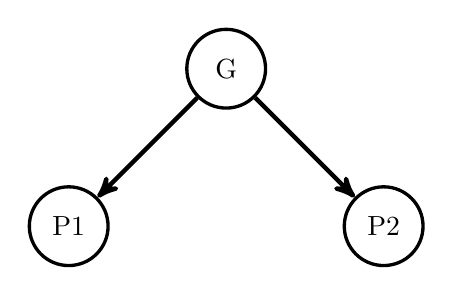
\begin{tikzpicture}[auto,node distance=.5cm,
    latent/.style={circle,draw,very thick,inner sep=0pt,minimum size=10mm,align=center},
    manifest/.style={rectangle,draw,very thick,inner sep=0pt,minimum width=45mm,minimum height=10mm},
    paths/.style={->, ultra thick, >=stealth'},
    twopaths2/.style={<->, ultra thick,bend left=90, >=stealth'},
    twopaths1/.style={<->, ultra thick,bend right=90, >=stealth'},
    mean/.style={draw, regular polygon, regular polygon sides=3, node distance=1cm, minimum height=10mm}
]

\node [latent] (G) at (0,0) {G};
\node [latent] (P1) at (-2,-2) {P1};
\node [latent] (P2) at (2,-2) {P2};

\draw [paths] (G.south west) to node [right] {} (P1);
\draw [paths] (G.south east) to node [right] {} (P2);

\end{tikzpicture}
} 
    \caption{Pleiotropy}\label{fig:pleiotropy}
  \end{subfigure}
  \begin{subfigure}[t]{0.5\textwidth}
    \centering
    \resizebox{0.5\linewidth}{!}{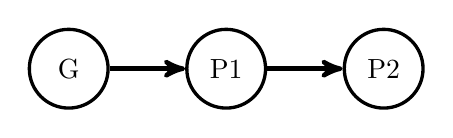
\begin{tikzpicture}[auto,node distance=.5cm,
    latent/.style={circle,draw,very thick,inner sep=0pt,minimum size=10mm,align=center},
    manifest/.style={rectangle,draw,very thick,inner sep=0pt,minimum width=45mm,minimum height=10mm},
    paths/.style={->, ultra thick, >=stealth'},
    twopaths2/.style={<->, ultra thick,bend left=90, >=stealth'},
    twopaths1/.style={<->, ultra thick,bend right=90, >=stealth'},
    mean/.style={draw, regular polygon, regular polygon sides=3, node distance=1cm, minimum height=10mm}
]

\node [latent] (G) at  (0,0) {G};
\node [latent] (P1) at (2,0) {P1};
\node [latent] (P2) at (4,0) {P2};

\draw [paths] (G.east) to node [right] {} (P1);
\draw [paths] (P1.east) to node [right] {} (P2);

\end{tikzpicture}
} 
    \caption{Mediated Pleiotropy}\label{fig:mediated_pleiotropy}
  \end{subfigure}
  \begin{subfigure}[t]{0.5\textwidth}
    \centering
    \resizebox{0.6\linewidth}{!}{
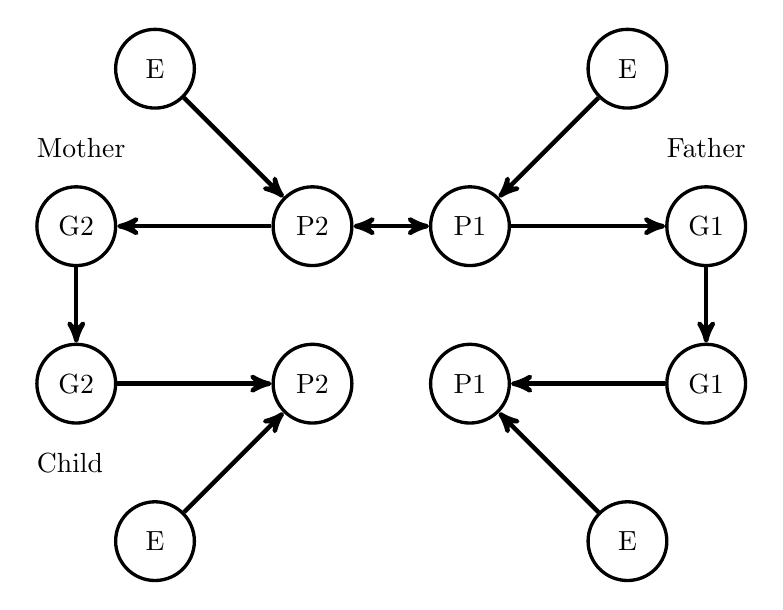
\begin{tikzpicture}[auto,node distance=.5cm,
    latent/.style={circle,draw,very thick,inner sep=0pt,minimum size=10mm,align=center},
    manifest/.style={rectangle,draw,very thick,inner sep=0pt,minimum width=45mm,minimum height=10mm},
    paths/.style={->, ultra thick, >=stealth'},
    paths2/.style={<->, ultra thick, >=stealth'},
    twopaths2/.style={<->, ultra thick,bend left=90, >=stealth'},
    twopaths1/.style={<->, ultra thick,bend right=90, >=stealth'},
    mean/.style={draw, regular polygon, regular polygon sides=3, node distance=1cm, minimum height=10mm}
]

\node [latent] (P2) at (0,0) {P2};
\node [latent] (P1) at (2,0) {P1};

\node [latent] (G1) at (5,0) {G1};
\node [latent] (G2) at (-3,0) {G2};

\node [latent] (E1) at (4,2) {E};
\node [latent] (E2) at (-2,2) {E};

\node [latent] (P1c) at (2,-2) {P1};
\node [latent] (P2c) at (0,-2) {P2};

\node [latent] (G1c) at (5,-2) {G1};
\node [latent] (G2c) at (-3,-2) {G2};

\node [latent] (E1c) at (4,-4) {E};
\node [latent] (E2c) at (-2,-4) {E};

\draw [paths] (P1.east) to node [right] {} (G1);
\draw [paths] (P2.west) to node [right] {} (G2);
\draw [paths] (G1.south) to node [right] {} (G1c);
\draw [paths] (G2.south) to node [right] {} (G2c);
\draw [paths] (E1.south west) to node [right] {} (P1);
\draw [paths] (E2.south east) to node [right] {} (P2);

\draw [paths] (G1c.west) to node [right] {} (P1c);
\draw [paths] (G2c.east) to node [right] {} (P2c);

\draw [paths] (E1c.north west) to node [right] {} (P1c);
\draw [paths] (E2c.north east) to node [right] {} (P2c);

\draw [paths2] (P1.west) to node [right] {} (P2.east);


\node [text width=1cm] at (5,1) {Father};
\node [text width=1cm] at (-3,1) {Mother};
\node [text width=1cm] at (-3,-3) {Child};

\end{tikzpicture}
} 
    \caption{Assortative Mating}\label{fig:assortative_mating}
  \end{subfigure}
  \begin{subfigure}[t]{0.5\textwidth}
    \centering
    \resizebox{0.6\linewidth}{!}{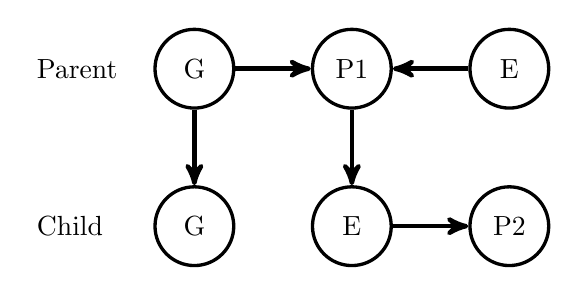
\begin{tikzpicture}[auto,node distance=.5cm,
    latent/.style={circle,draw,very thick,inner sep=0pt,minimum size=10mm,align=center},
    manifest/.style={rectangle,draw,very thick,inner sep=0pt,minimum width=45mm,minimum height=10mm},
    paths/.style={->, ultra thick, >=stealth'},
    twopaths2/.style={<->, ultra thick,bend left=90, >=stealth'},
    twopaths1/.style={<->, ultra thick,bend right=90, >=stealth'},
    mean/.style={draw, regular polygon, regular polygon sides=3, node distance=1cm, minimum height=10mm}
]

\node [latent] (Gp) at (0,0) {G};
\node [latent] (P1) at (2,0) {P1};
\node [latent] (Ep) at  (4,0) {E};
\node [latent] (Gc) at (0,-2) {G};
\node [latent] (Ec) at  (2,-2) {E};
\node [latent] (P2) at (4,-2) {P2};

\node [text width=1cm] at (-1.5,0) {Parent};
\node [text width=1cm] at (-1.5,-2) {Child};

\draw [paths] (Gp.east) to node [right] {} (P1);
\draw [paths] (Gp.south) to node [right] {} (Gc);
\draw [paths] (P1.south) to node [right] {} (Ec);
\draw [paths] (Ep.west) to node [right] {} (P1);
\draw [paths] (Ec.east) to node [right] {} (P2);

\end{tikzpicture}
}
    \caption{Parental Effects}\label{fig:parental_effects}
  \end{subfigure}
  \caption{Different sources of genetic correlation according to~\citet{Pickrell2016}}\label{fig:genetic_correlation}
\end{figure}

To conclude, during the last few years large gains have been made in fostering our understanding of heritability and genetic correlations with the development of GCTA and LD-score.
While these tools are able to estimate heritability and genetic correlations of a number of traits it remains difficult to distinguish between different sources of genetic correlations.

\section{Association studies on rare variants}
\label{sec:association_studies_on_rare_varitants}

A possible suspect for the missing heritability are rare variants.
Rare variants, commonly variants with a \acrfull{maf} of equal or below 1\%, have been suggested to explain the bulk of missing heritability~\cite{Jiang2013,Li2009a}.
Rare variants are commonly not accessible via micro array chips but only via the more cost intensive sequencing.
However, the drop in sequencing costs has allowed to conduct whole-exome and whole genome association studies or rare variants~\cite{Goodwin2016}.
In contrast to GWASs, single variants associations are largely unfeasible, unless sample size is very large~\cite{Lee2014}.
Hence, considerable effort has been made to develop and deploy statistical methods to improve statistical power of rare variant association studies~\cite{Morris2010,Zeng2014,Daye2012,Manuscript2013}.
Instead of testing individual genetic markers most statistical test evaluate the combined effect of multiple genetic variations in a biological relevant region, such as a gene.
In general one can divide such approaches into burden and variance component tests.
I will first introduce the general statistical model for the two tests.
Following I will outline each test class and evaluate their benefits and drawbacks.

Assuming that $y_i$ for subject $i$ with mean $\mu_i$ follows a distribution in the quasi-likelihood family~\cite{Lee2014} with $n$ subjects in a region with $m$ variants, then
\begin{equation}
  h(\mu_i) = \alpha_0 + \alpha'X_i +\beta'G_i
\end{equation}
in which $h(\mu) = \mu$ or $h(\mu) = logit(\mu)$.
The regression coefficients of the covariants and allele counts are $\alpha = (\alpha_1, \ldots, \alpha_q)$ as well as $\beta = (\beta_1, \ldots, \beta_m)$ respectively.
The covariants are denoted as $X_i = (X_{i1}, \ldots, X_{iq})'$ and the allele counts as $G_{i1}, \ldots, G_{im}$.
The score statistic of the marginal model for variant $j$ is then
\begin{equation}
  S_j = \sum^n_{i=1} G_{ij}(y_i-\hat{\mu_i})
\end{equation}
where $\hat{\mu_i}$ is the estimated mean under $H_0: \beta = 0 $ and is obtained by $h(\mu_i) = \alpha_0 + \alpha'X_i$.

\subsection{Burden Test}
\label{sub:burden_test}
The simplest approach, called the burden test, tests the weighted sum of commutated scores
\begin{equation}\label{eq:burden}
  Q = {(\sum^{m}_{j=1} w_{j} S_{j})}^2
\end{equation}
in which $w_j$ is the weight for variant $j$.
Weights can be define by functional annotations, allele frequency or others.
The test assumes that all variants  have the same direction of effect.
This is a rather strong assumption and violations result in a loss in statistical power~\cite{Derkach2013a}.

\subsection{Variance Component Tests}
\label{sub:variance_component_tests}
In contrast to burden tests variance-component tests evaluate the distribution of effects within a certain genomic region.
The most prominent member of this test family is SKAT~\cite{Wu2011}.
SKAT assume that $\beta_j\sim N(0,w_j\tau)$ and test for $H_0: \tau = 0$ with a variance-component score test.
The test statistic is defined as
\begin{equation}\label{eq:skat}
  Q = \sum^{m}_{j=1} w_{j}^2 S_{j}^2
\end{equation}
The test is robust to groupings of protective and damaging effects within the same region.
However, also SKAT suffer from a reduction in statistical power in cases of high proportions of causal variants with the same direction~\cite{Derkach2013a}.

To summarise, variance-component tests are generally more powerful than burden tests if a region has many non-causal variants or when the effects of a genomic regions are bi-directional.
In contrast burden tests perform better in scenarios where most causal variants have the same direction of effect.
This has led to the development of omnibus tests to combine burden and variance component tests, most notably SKAT-O~\cite{Lee2012}.
\bigskip

To conclude, I have outlined various statistical methods to investigate the genetic contribution of aggressive behavior.
I have described the commonly applied twin model to estimate the contribution of genetic and environmental effects.
Further, I outlined the principles of genome wide association studies as well as the use of GCTA and LD-score to estimate the narrow sense heritability from common SNPs.
At last I have described two common used rare variant tests as well as their pros and cons.

In the next chapter I will present an investigation of the longitudinal heritability of childhood aggression with the use of two large twin cohorts. 
\end{document}

\end{document}
